\documentclass[journal]{IEEEtran}
% ============================================================================
% When Does a Kolmogorov-Arnold Network Help in Wireless?
% A parameter-matched, non-saturated benchmark. Honest-measurement research paper.
% All numbers are traced to ../code results via claims.json (verify_numbers.py).
% ============================================================================
\usepackage{amsmath,amssymb}
\usepackage{graphicx}
\usepackage{booktabs}
\usepackage{url}
\usepackage[hidelinks]{hyperref}
\graphicspath{{figs/}}

\begin{document}
\title{When Do Kolmogorov--Arnold Networks Help in Wireless?\\
A Matched-Capacity, Non-Saturated Benchmark}

\author{Do Phuc Hao%
\thanks{D. P. Hao is with Da Nang Architecture University, Da Nang, Vietnam
(email: haodp@dau.edu.vn).}%
\thanks{Manuscript submitted to the IEEE Transactions on Cognitive Communications and
Networking, August 2026. Code and data-preparation scripts that reproduce every reported
number are released (Section~\ref{sec:repro}).}}

\markboth{IEEE Transactions on Cognitive Communications and Networking (Submitted, August 2026)}%
{Do: When Do Kolmogorov--Arnold Networks Help in Wireless?}

\maketitle

\begin{abstract}
Kolmogorov--Arnold networks (KANs) are increasingly proposed for wireless tasks with two
claims: they match or beat multilayer perceptrons (MLPs) at fewer parameters, and their
learned univariate edge functions make them interpretable. Rather than accept or dismiss
these claims, we map \emph{when} they hold, using a parameter-matched, multi-seed protocol
on three non-saturated wireless regimes: power-amplifier behavioral modeling, OFDM channel
estimation, and automatic modulation classification on the real RML2016.10a dataset. The honest picture is regime-dependent. KANs are genuinely competitive and
sometimes better: a spline-KAN beats a matched MLP on modulation classification above about
$2$~dB SNR and across the full SNR range, a Fourier-KAN with a richer basis beats the MLP on
the regression task at matched capacity, and KANs win in the low-data regime. But the two most
common KAN variants never dominate: a small, task-appropriate convolutional network beats every
flat model on classification by a wide margin at a fraction of the parameters, at the default
budget a plain MLP is the stronger flat model at low SNR, and a properly built classical model
ties or beats the KANs on regression. An interpretability audit shows the KAN's edges are
simple (a cubic fits them with median $R^2=0.998$), yet the symbolic extraction that would make
them interpretable costs over a decibel, so the readable model is not the performant one. We
conclude that the sweeping KAN ``efficiency wins'' reported for wireless track unmatched
capacity and favorable benchmarks, give a regime map of where KANs actually help, and release a
reusable protocol and harness.
\end{abstract}

\begin{IEEEkeywords}
Kolmogorov--Arnold networks, wireless machine learning, modulation classification,
digital predistortion, model interpretability, benchmarking.
\end{IEEEkeywords}

% ============================================================================
\section{Introduction}\label{sec:intro}
% ============================================================================
\IEEEPARstart{K}{olmogorov}--Arnold networks (KANs)~\cite{liu2024kan} replace the fixed
node nonlinearities of a multilayer perceptron (MLP) with \emph{learnable} univariate
functions on the edges, parameterized by splines~\cite{liu2024kan} or truncated Fourier
series~\cite{efficientkan}. Two properties are repeatedly advertised: a favorable
accuracy-per-parameter trade-off against MLPs, and interpretability, because the learned
one-dimensional edge functions can in principle be read off and replaced by closed-form
symbols. Within roughly a year these claims have propagated into wireless communications:
KANs have been proposed for modulation recognition, channel estimation, digital
predistortion (DPD)~\cite{kandpd}, radio-frequency fingerprinting~\cite{kanrff},
and 6G signal intelligence~\cite{wsr6g}.

The wireless literature, however, has adopted KANs largely in a \emph{showcase} mode: a
KAN is shown to beat some baseline on some task, and the advantage is attributed to the
architecture. Two methodological problems make such claims hard to trust, and both are
known in the broader machine-learning community~\cite{yu2024fairer}. First,
\textbf{capacity is rarely matched}: a small KAN is compared against a differently sized
MLP, so ``fewer parameters'' can be an artifact of the comparison rather than a property
of the model. Second, \textbf{benchmarks are often saturated}: when every model already
exceeds, say, $99\%$ accuracy, differences are within noise and the comparison cannot
distinguish architectures at all. A recent survey of KANs~\cite{kansurvey2024} and a
fairness study on vision and tabular tasks~\cite{yu2024fairer} both caution that KAN
advantages shrink or vanish once these controls are applied, but the question has not
been asked cleanly \emph{for wireless}, where the tasks, inductive biases, and baselines
differ.

This paper asks the question directly and answers it with measurement. We do not propose
a new architecture; we propose an honest evaluation and report what it shows, whichever
way it falls. Concretely:

\begin{itemize}
\item We define a \textbf{parameter-matched, multi-seed benchmarking protocol}
(Section~\ref{sec:protocol}) in which KANs and baselines are sized to the same parameter
budget, trained identically, and compared with bootstrap confidence intervals and paired
differences. Baselines are chosen to be \emph{strong and task-appropriate}, not
strawmen.
\item We evaluate three wireless regimes chosen to be \textbf{non-saturated}, so
differences are resolvable: (i) power-amplifier behavioral modeling / DPD, a smooth
low-dimensional regression that is the regime most favorable to KANs (Section~\ref{sec:dpd});
(ii) automatic modulation classification (AMC) on the real RML2016.10a dataset
(Section~\ref{sec:amc}); and (iii) OFDM channel estimation, an estimation task with a
strong LMMSE baseline (Section~\ref{sec:chest}).
\item We conduct an \textbf{interpretability audit} (Section~\ref{sec:interp}) that
separates two things a claim of interpretability must satisfy: are the learned edges
simple, and is the simple form free? We find the edges are simple but the symbolic
distillation that realizes the interpretability claim degrades accuracy.
\item We run \textbf{ablations} (Section~\ref{sec:abl}) that stress-test the comparison in
KAN's favor: parameter-budget, \emph{symmetric} KAN-and-MLP hyperparameter, training-set-size,
and SNR sweeps. These reveal honest crossovers, KANs win in some regimes, and pin down where.
\item We audit \textbf{computational cost} (Section~\ref{sec:compute}): at matched parameters,
KANs are $4$ to $30\times$ slower per inference than the MLP, so the ``efficiency'' that
motivates them is largely illusory once compute, not just parameter count, is measured.
\item We synthesize a \textbf{regime map} and practical guidance
(Section~\ref{sec:discuss}): KANs are competitive and win in specific regimes
(high-SNR classification, low data, richer bases) but never dominate, are beaten by the
right inductive bias, and carry a measurable interpretability cost. We release all code
(Section~\ref{sec:repro}).
\end{itemize}

Our aim is neither to promote nor to dismiss KANs, but to replace showcase claims with a
regime map: to show precisely where the imported value propositions hold and where they do
not, and to give the community a protocol that surfaces this before a claim is believed.

% ============================================================================
\section{Background and Related Work}\label{sec:bg}
% ============================================================================
\subsection{Kolmogorov--Arnold networks}
KANs are motivated by the Kolmogorov--Arnold representation theorem~\cite{kolmogorov1957},
which states that any multivariate continuous function can be written as a finite
composition of continuous univariate functions and addition. Where the classical
universal-approximation results for MLPs~\cite{cybenko1989,hornik1991} place the
nonlinearity at the nodes and learn linear edge weights, KANs~\cite{liu2024kan,liu2024kan2}
invert this: the edges carry learnable univariate functions and the nodes merely sum. A
KAN layer maps $\mathbf{x}\in\mathbb{R}^{d_{\mathrm{in}}}$ to
$\mathbf{y}\in\mathbb{R}^{d_{\mathrm{out}}}$ through a learnable univariate function on
each edge:
\begin{equation}
y_j = \sum_{i=1}^{d_{\mathrm{in}}} \phi_{ji}(x_i) + b_j ,
\end{equation}
where each $\phi_{ji}$ is a spline~\cite{liu2024kan} or a truncated Fourier
series~\cite{efficientkan}. The spline variant we use follows the standard
efficient formulation~\cite{efficientkan}: $\phi_{ji}(x)=w^{b}_{ji}\,\mathrm{silu}(x) +
\sum_{c} w^{s}_{jic} B_c(x)$, with $B_c$ the B-spline basis on a fixed grid. The Fourier
variant uses $\phi_{ji}(x)=\sum_{k=1}^{K}\big[a_{jik}\cos(kx)+b_{jik}\sin(kx)\big]$.
Both give a per-layer parameter count of the form $d_{\mathrm{in}} d_{\mathrm{out}}\,C$,
where $C$ is the per-edge coefficient count; this is the quantity we hold fixed when we
speak of a matched budget. A rapidly growing family of variants swaps the edge basis
(wavelets in Wav-KAN~\cite{wavkan}, Gaussian radial bases in FastKAN~\cite{fastkan},
Chebyshev polynomials in Cheby-KAN~\cite{chebykan}), and recent work also examines the
hardware inference cost of these choices~\cite{hwkan2026}; none changes the parameter
accounting above, so our matched-budget comparison of the two most common instantiations,
spline and Fourier, is representative. We use PyTorch implementations~\cite{paszke2019pytorch}
following the efficient spline formulation~\cite{efficientkan}.

\subsection{KAN claims and their audits}
The original proposal~\cite{liu2024kan} emphasizes accuracy-per-parameter on scientific
regression and symbolic-regression interpretability. Subsequent scrutiny is mixed:
\cite{yu2024fairer} finds that under a fair comparison KANs beat MLPs mainly on symbolic
formula tasks and often lose on vision and tabular data, and a broad survey~\cite{kansurvey2024}
catalogues the fast-growing but largely showcase-style application literature. The
interpretability claim in particular is usually asserted qualitatively (a plot of a few
edges) rather than tested for fidelity. This matters because interpretability in machine
learning is a substantive property, not a byproduct of a readable plot: the literature
distinguishes genuinely interpretable models from post-hoc explanations of black
boxes~\cite{rudin2019,molnar2020,lundberg2017shap}, and the question of whether a simpler
surrogate preserves a model's behavior is exactly the subject of knowledge distillation and
model-compression studies~\cite{hinton2015distill,ba2014deep}. Our fidelity audit
(Section~\ref{sec:interp}) applies that lens to KAN's symbolic-extraction claim.

\subsection{KANs in wireless}
Deep learning is now pervasive in the wireless physical layer~\cite{oshea2017intro,lecun2015deep},
and KAN adoption there is recent and application-driven. For DPD, several KAN and symbolic-KAN
models have been proposed to linearize power amplifiers with reduced
complexity~\cite{kandpd,kandpd_rof,etdkan}; for radio-frequency fingerprinting,
KAN-augmented residual networks report identification gains~\cite{kanrff}; and
signal-intelligence surveys for 6G list KANs among emerging tools alongside large language
models~\cite{wsr6g,radiollm}. Across these works, the comparison is typically against an
unmatched MLP or a single baseline, and the benchmark is not checked for saturation. The
tasks themselves are well studied independently: AMC on the RML2016 datasets~\cite{oshea2016conv,oshea2016gnuradio,oshea2018over}
is a standard classification benchmark, best attacked with convolutional inductive
bias~\cite{krizhevsky2012}, whose low-SNR band remains far from saturation~\cite{rml22,fsosamc};
PA behavioral modeling has a mature classical baseline in the memory polynomial and its
generalizations~\cite{ding2004mempoly,morgan2006gmp,saleh1981}; and richer real-world
benchmarks such as DeepSense~6G~\cite{deepsense6g} confirm that many wireless tasks are far
from solved. Interpretable-AI work for the physical layer~\cite{xaichannel} motivates the
interpretability question but does not quantify KAN fidelity. Our contribution is to place
KANs on these tasks under a matched-capacity, non-saturated, multi-seed protocol and to
audit interpretability quantitatively.

% ============================================================================
\section{Benchmarking Protocol}\label{sec:protocol}
% ============================================================================
The protocol (Fig.~\ref{fig:protocol}) exists to remove the two confounds identified in
Section~\ref{sec:intro}. It has four rules.

\begin{figure}[t]
\centering
\includegraphics[width=0.86\columnwidth]{fig_protocol.pdf}
\caption{The honest benchmarking protocol: fix a parameter budget, size every model to it,
train identically over multiple seeds, and report bootstrap intervals and paired differences
on a non-saturated regime. Baselines are strong and task-appropriate.}
\label{fig:protocol}
\end{figure}

\emph{(1) Matched capacity.} For each task we fix a target parameter budget $P$ and size
every model to it. For a two-layer network with input width $d$, hidden width $h$, and output
width $c$, the parameter counts are
\begin{align}
P_{\mathrm{MLP}} &= dh + h^2 + hc + (2h+c), \label{eq:pmlp}\\
P_{\mathrm{KAN}}^{\mathrm{F}} &= 2K\,(dh + hc) + (h+c), \label{eq:pkanf}\\
P_{\mathrm{KAN}}^{\mathrm{S}} &= (1{+}G{+}k)\,(dh + hc), \label{eq:pkans}
\end{align}
where $K$ is the Fourier order and $(G,k)$ the spline grid and degree. The trendy factor
$2K$ or $(1{+}G{+}k)$ multiplies the same $dh{+}hc$ connectivity, so a KAN and an MLP reach the
same $P$ only at different hidden widths. We fix the Fourier-KAN, compute its $P$ from
\eqref{eq:pkanf}, and solve \eqref{eq:pmlp} and \eqref{eq:pkans} for the MLP and spline-KAN
widths that land within a few percent of it. This makes ``KAN uses fewer parameters'' testable
rather than assumed. For DPD all learned models sit at $P\approx\input{claims/dpd_params}$
parameters; the residual mismatch is under $3\%$.

\emph{(2) Strong, task-appropriate baselines.} A KAN must be compared against the
baseline a practitioner would actually use. For the smooth regression regime that is a
memory polynomial fit by regularized least squares~\cite{morgan2006gmp}, the classical DPD
workhorse; we condition its basis so it is not a strawman. For the structured
classification regime it is a small convolutional network that exploits the I/Q time
structure. The matched MLP is the fairness control common to both.

\emph{(3) Multiple seeds and interval estimates.} Each configuration is trained over
several seeds (five for the regression regime, ten for classification); throughout, $\pm$
denotes one standard deviation across seeds, and bracketed intervals are bootstrap $95\%$
confidence intervals of the mean. For the head-to-head question we report the \emph{paired}
KAN-minus-baseline difference with its own bootstrap interval, and call a difference
significant only when that interval excludes zero. No result rests on a single seed.

\emph{(4) Non-saturated regimes.} We deliberately choose operating points where no model
is near the ceiling, so a real difference can appear. This is the opposite of the common
practice of reporting on a band where every model exceeds $99\%$.

Both KAN variants, the MLP, the CNN, and the memory-polynomial baseline are implemented in
a single harness so that training schedule, optimizer, and data pipeline are identical
across models; only the architecture changes. All neural models are trained with the Adam
optimizer~\cite{kingma2015adam} under a cosine learning-rate schedule and identical epoch
budgets, and the memory-polynomial baseline is fit by regularized least squares. Table~\ref{tab:arch}
summarizes the models and how each is sized to the shared budget.

\begin{table}[t]
\centering
\caption{Models and matched-capacity sizing. Each learned model is sized to the shared
per-task budget $P$; the CNN is included as the strong structural baseline for AMC.}
\label{tab:arch}
\begin{tabular}{lll}
\toprule
Model & Edge / layer function & Sized by \\
\midrule
KAN (spline)  & B-spline on each edge      & hidden width \\
KAN (Fourier) & truncated Fourier per edge & width, order $K$ \\
MLP           & linear + ReLU nodes        & hidden width \\
CNN           & 1-D conv.\ over I/Q        & fixed (small) \\
mem.\ poly.   & $x|x|^{k-1}$ basis, LS fit & memory, order \\
\bottomrule
\end{tabular}
\end{table}

% ============================================================================
\section{Regime 1: PA Behavioral Modeling (DPD)}\label{sec:dpd}
% ============================================================================
\subsection{Task and data}
Power-amplifier (PA) behavioral modeling is a smooth, low-dimensional nonlinear regression
and is the regime KANs are \emph{claimed} to handle best, since each edge can in principle
capture a one-dimensional AM/AM-like curve. We drive a Wiener--Hammerstein PA with a
pulse-shaped 16-QAM baseband signal at $6$~dB input backoff. With input FIR $h_1$, output FIR
$h_2$, and $u[n]=(h_1{*}x)[n]$, the static Saleh nonlinearity~\cite{saleh1981} applies
amplitude and phase distortion
\begin{equation}
A(r)=\frac{\alpha_a r}{1+\beta_a r^2},\qquad
\Phi(r)=\frac{\alpha_p r^2}{1+\beta_p r^2},
\label{eq:saleh}
\end{equation}
so that the PA output is
\begin{equation}
y[n]=\Big(h_2*v\Big)[n],\quad
v[n]=A(|u[n]|)\,e^{\,j\big(\angle u[n]+\Phi(|u[n]|)\big)} .
\label{eq:wh}
\end{equation}
Because \eqref{eq:saleh}--\eqref{eq:wh} is not a memory polynomial, the classical
memory-polynomial baseline gets no unfair ``true model class'' advantage; all learners
approximate. The task is to predict the complex PA output $y[n]$ from a length-$M{=}5$ memory
window of the complex input, and the metric throughout the paper is the normalized
mean-squared error
\begin{equation}
\mathrm{NMSE}=10\log_{10}\frac{\sum_n \lVert \hat{y}[n]-y[n]\rVert^2}{\sum_n \lVert y[n]\rVert^2}\ \text{[dB]} .
\label{eq:nmse}
\end{equation}
Models are trained over $5$ seeds. We evaluate \emph{behavioral modeling}, the forward-model accuracy
that a predistorter is built on, rather than a full indirect-learning DPD loop; we therefore
report NMSE and not ACPR or EVM, and read the results as a statement about learning a smooth
PA nonlinearity, not about end-to-end linearization. Because the ground-truth PA is a Saleh
model, its AM/AM curve is smooth by construction; a measured PA with strong memory or
hysteresis could shift the boundaries, as we note in Section~\ref{sec:discuss}.

\subsection{Results}
Table~\ref{tab:dpd} and Fig.~\ref{fig:dpd} report the outcome. At a matched budget of
$\input{claims/dpd_params}$ parameters, the plain MLP achieves the best NMSE,
$\input{claims/dpd_mlp_nmse}$~dB, beating the Fourier-KAN
($\input{claims/dpd_kanfourier_nmse}$~dB) and the canonical spline-KAN
($\input{claims/dpd_kanspline_nmse}$~dB). The paired differences are
$+\input{claims/dpd_kanfourier_minus_mlp}$~dB (Fourier-KAN worse than MLP) and
$+\input{claims/dpd_kanspline_minus_mlp}$~dB (spline-KAN worse than MLP); both confidence
intervals exclude zero, so the MLP advantage is significant. Crucially, the classical baseline
is not a strawman: a properly built generalized memory polynomial (GMP)~\cite{morgan2006gmp},
\begin{equation}
\hat{y}[n]=\!\!\sum_{\substack{k\ \mathrm{odd}}}\ \sum_{m}\ \sum_{|m'-m|\le 2}\!\!
c_{k,m,m'}\;x[n{-}m]\,\bigl|x[n{-}m']\bigr|^{k-1},
\label{eq:gmp}
\end{equation}
with the lagging/leading cross-envelope terms $m'\neq m$ that a diagonal memory polynomial
omits, reaches $\input{claims/dpd_mempoly_nmse}$~dB, statistically tied with the best neural
model and better than both KANs. So at the \emph{default} matched configuration, even on the regime most
favorable to KANs, the KANs beat neither a same-budget MLP nor the right classical method,
and the widely used spline-KAN is the worst option of all. This ranking is not the whole
story, however: Section~\ref{sec:abl} shows that a Fourier-KAN with a richer basis overtakes
the MLP at matched capacity, and that KANs win when training data is scarce. The point of the
default result is only that KAN superiority is not automatic; it must be earned and measured.

\begin{table}[t]
\centering
\caption{DPD / PA modeling, matched capacity, 5 seeds. NMSE in dB (lower is better).}
\label{tab:dpd}
\begin{tabular}{lrr}
\toprule
Model & Params & NMSE [dB] $\downarrow$ \\
\midrule
MLP (matched)        & $2354$ & $\mathbf{-16.27\pm0.12}$ \\
GMP (classical)      & --     & $-16.20\pm0.05$ \\
KAN, Fourier         & $2330$ & $-15.50\pm0.06$ \\
KAN, spline (canon.) & $2280$ & $-14.09\pm0.08$ \\
\bottomrule
\end{tabular}
\end{table}

\begin{figure}[t]
\centering
\includegraphics[width=\columnwidth]{fig_dpd.pdf}
\caption{DPD regime, matched capacity. A same-budget MLP achieves the best modeling NMSE;
both KAN variants are worse (paired differences $0.8$--$2.2$~dB, intervals exclude zero).}
\label{fig:dpd}
\end{figure}

% ============================================================================
\section{Regime 2: Modulation Classification (RML2016.10a)}\label{sec:amc}
% ============================================================================
\subsection{Task and data}
Automatic modulation classification is a high-dimensional, structured-input classification
task. We use the real RML2016.10a dataset~\cite{oshea2016gnuradio}, which contains $128$-sample
complex I/Q frames over $11$ modulations and a range of SNRs. We restrict to the
\emph{low-SNR band} from $\input{claims/amc_snr_lo}$ to $\input{claims/amc_snr_hi}$~dB,
where accuracy is far from saturation and model differences are resolvable, and draw
$\input{claims/amc_n}$ power-normalized frames. The flat models see the $256$-dimensional
flattened I/Q vector; the CNN sees the $2\times128$ frame. Models are trained over
$\input{claims/n_seeds_amc}$ seeds.

\subsection{Results}
Table~\ref{tab:amc} and Fig.~\ref{fig:amc} report the outcome. The small convolutional
baseline, with only $5291$ parameters, reaches
$\input{claims/amc_cnn_acc}$ accuracy and dominates every flat model. Among the flat
models at a matched budget of about $68$k parameters, the MLP
($\input{claims/amc_mlp_acc}$) again beats both KANs; the spline-KAN
($\input{claims/amc_kanspline_acc}$) is close but below, and the Fourier-KAN
($\input{claims/amc_kanfourier_acc}$) is markedly worse. The paired Fourier-KAN-minus-MLP
difference is $\input{claims/amc_kanfourier_minus_mlp}$ (KAN worse), and the CNN leads the
best KAN by $+\input{claims/amc_cnn_minus_kanfourier}$; both intervals exclude zero. One
lesson is unconditional and mirrors nothing in the regression regime: the right inductive
bias, a convolution over the I/Q sequence, beats all flat models by a wide margin at a
fraction of the parameters. The MLP-over-KAN ordering, however, is specific to this low-SNR
band, and it inverts elsewhere: the SNR sweep in Section~\ref{sec:abl} shows the spline-KAN
overtaking the MLP above about $\input{claims/snr_crossover_db}$~dB and across the full SNR
range, so our choice of the hardest band, made to avoid saturation, happens to be where the
MLP looks best. This is exactly why an honest benchmark must resolve the operating point
rather than report a single aggregate.

\begin{table}[t]
\centering
\caption{AMC on RML2016.10a, low-SNR band $[-6,6]$~dB, matched flat-model capacity,
10 seeds. Accuracy (higher is better).}
\label{tab:amc}
\begin{tabular}{lrr}
\toprule
Model & Params & Accuracy $\uparrow$ \\
\midrule
CNN (task-appropriate) & $5291$  & $\mathbf{0.658\pm0.005}$ \\
MLP (matched)          & $68651$ & $0.495\pm0.003$ \\
KAN, spline (canon.)   & $69420$ & $0.468\pm0.006$ \\
KAN, Fourier           & $68395$ & $0.349\pm0.007$ \\
\bottomrule
\end{tabular}
\end{table}

\begin{figure}[t]
\centering
\includegraphics[width=\columnwidth]{fig_amc.pdf}
\caption{AMC regime (real RML2016.10a, low-SNR). A small CNN dominates; among matched flat
models the MLP beats both KANs. The correct inductive bias, not the edge parameterization,
decides the task.}
\label{fig:amc}
\end{figure}

\subsection{Where the KAN advantage lives}
To locate the KAN advantage we resolve accuracy by modulation on the mid-band ($0$ to
$12$~dB), the regime where the SNR sweep places the spline-KAN ahead of the MLP; this
decomposes the high-SNR crossover, not the low-SNR headline of Table~\ref{tab:amc}, and we
report it as such. In this regime (Fig.~\ref{fig:permod}) the spline-KAN's advantage over the
matched MLP is not spread evenly: it concentrates on the phase- and amplitude-shift
modulations whose decision regions are constellation geometry, gaining
$+\input{claims/permod_kan_bpsk_gain}$ on BPSK, $+\input{claims/permod_kan_pam4_gain}$ on PAM4,
and $+\input{claims/permod_kan_8psk_gain}$ on 8PSK, while it slightly trails the MLP on the
analog and frequency-modulated classes (for example $\input{claims/permod_kan_gfsk_loss}$ on
GFSK). This pattern is consistent with, though it does not prove, a per-edge mechanism: a
learnable univariate function per input can carve the smooth amplitude/phase boundaries of a
constellation, but offers little for signals whose class is carried by frequency dynamics that
a flat model reads only weakly in any case. The KAN is thus not a generically better
classifier; where it helps, it is a better fit to a specific, identifiable structure.

\begin{figure}[t]
\centering
\includegraphics[width=\columnwidth]{fig_permod.pdf}
\caption{Per-modulation accuracy difference, spline-KAN minus matched MLP, on the mid-band
($0$ to $12$~dB) where the KAN leads overall. The KAN advantage concentrates on
constellation-geometry modulations (BPSK, PAM4, 8PSK, QPSK) and reverses on frequency/analog
modulations, consistent with a per-edge decision-boundary mechanism.}
\label{fig:permod}
\end{figure}

% ============================================================================
\section{Regime 3: OFDM Channel Estimation}\label{sec:chest}
% ============================================================================
To test a third, structurally different task, we add OFDM channel estimation: an
\emph{estimation} problem rather than PA modeling or classification. On an $N{=}\input{claims/chest_subcarriers}$
subcarrier grid with $L{=}8$ multipath taps (exponential power-delay profile), comb pilots
observe the channel frequency response at $\input{claims/chest_pilots}$ subcarriers under noise
at $\input{claims/chest_snr_db}$~dB SNR, and the task is to estimate the channel at all
subcarriers. The metric is channel NMSE in dB, over $5$ seeds. The decisive point is the
baseline: linear minimum mean-square error (LMMSE) estimation is the Wiener estimator, optimal
in the linear-Gaussian setting, and is the genuine classical workhorse here. From the noisy
pilot observations $\mathbf{y}_p=\mathbf{H}_p+\mathbf{n}$ it forms
\begin{equation}
\hat{\mathbf{H}}=\mathbf{R}_{H H_p}\bigl(\mathbf{R}_{H_p H_p}+\sigma^2\mathbf{I}\bigr)^{-1}\mathbf{y}_p,
\label{eq:lmmse}
\end{equation}
with $\mathbf{R}_{H H_p}$ and $\mathbf{R}_{H_p H_p}$ the channel cross- and pilot
auto-covariances estimated from training; we also include simple linear interpolation as a weak
reference.

Table~\ref{tab:chest} and Fig.~\ref{fig:chest} report the result. The classical LMMSE is the
best estimator at $\input{claims/chest_lmmse_nmse}$~dB, ahead of every neural model. Among the
neural models the spline-KAN ($\input{claims/chest_kanspline_nmse}$~dB) exactly ties the matched
MLP ($\input{claims/chest_mlp_nmse}$~dB), the Fourier-KAN
($\input{claims/chest_kanfourier_nmse}$~dB) is marginally behind, and all three clear the
linear-interpolation reference ($\input{claims/chest_lininterp_nmse}$~dB) by a wide margin. As
in the PA-modeling regime, the KAN buys nothing over a same-size MLP, and the right classical
method is not beaten by either. Three regimes, three task types, and the same conclusion at the
default configuration: KANs are competitive but not superior, and never beat the appropriate
classical or structural baseline.

\begin{table}[t]
\centering
\caption{OFDM channel estimation at $10$~dB SNR, matched capacity, 5 seeds. NMSE in dB
(lower is better).}
\label{tab:chest}
\begin{tabular}{lr}
\toprule
Model & NMSE [dB] $\downarrow$ \\
\midrule
LMMSE (classical)    & $\mathbf{-13.37\pm0.01}$ \\
MLP (matched)        & $-13.28\pm0.01$ \\
KAN, spline (canon.) & $-13.28\pm0.01$ \\
KAN, Fourier         & $-13.12\pm0.01$ \\
linear interpolation & $-9.48\pm0.01$ \\
\bottomrule
\end{tabular}
\end{table}

\begin{figure}[t]
\centering
\includegraphics[width=\columnwidth]{fig_chest.pdf}
\caption{Channel estimation, matched capacity. Classical LMMSE is the best estimator; the
spline-KAN exactly ties the matched MLP and neither beats LMMSE, mirroring the PA-modeling
regime on a different task type.}
\label{fig:chest}
\end{figure}

% ============================================================================
\section{Interpretability Audit}\label{sec:interp}
% ============================================================================
The second KAN claim is interpretability: the learned univariate edges are simple enough
to read off and replace by closed-form symbols, yielding an interpretable model ``for
free.'' A claim of this kind must satisfy two conditions, and we test them separately on
the DPD KAN, where the task is smooth and thus most favorable to the claim.

\emph{(Q1) Simplicity.} Are the learned first-layer edge functions well approximated by a
human-readable low-order polynomial? We sample each edge on its input support and fit a
cubic (over $5$ seeds). The fits are excellent: the median per-edge $R^2$ is
$\input{claims/interp_median_r2}$ and $\input{claims/interp_frac_simple_pct}\%$ of edges
exceed $R^2=0.95$ (Fig.~\ref{fig:interp}). To guard against near-flat edges inflating this,
we also weight each edge's $R^2$ by its function variance; the variance-weighted mean is
$\input{claims/interp_vw_r2}$, so the high-amplitude edges that actually carry the model are
simple too, not just the negligible ones. Fig.~\ref{fig:edges} makes this concrete by
overlaying three representative learned edges, spanning the best, median, and worst fits, on
their cubics: the dashed fits sit essentially on top of the solid curves, and the
highest-magnitude edge is a simple monotonic S-shape reminiscent of an AM/AM characteristic.
The edges are indeed simple; the claim is not vacuous.

\begin{figure}[t]
\centering
\includegraphics[width=\columnwidth]{fig_edges.pdf}
\caption{Three representative learned KAN edge functions (solid) and their cubic fits
(dashed), spanning the best, median, and worst per-edge fit. The fits are nearly coincident,
confirming the edges are simple, readable curves. Note the near-flat median and worst-fit
edges carry little of the model, which is why the variance-weighted $R^2$ is reported.}
\label{fig:edges}
\end{figure}

\emph{(Q2) Fidelity: is it free?} We then \emph{distill} the first layer into those cubics (a
symbolic surrogate), keep the rest of the network exact, and re-measure NMSE over the same
$5$ seeds. The surrogate degrades NMSE by $\input{claims/interp_degradation_db}\pm\input{claims/interp_degradation_std}$~dB.
In other words, the readable form is not the performant form: extracting the interpretable
symbols discards more than a decibel of modeling accuracy, consistently across seeds. Because
we symbolize only the first layer, this is a \emph{lower bound} on the cost of a fully
symbolic KAN, and a task-loss-refit surrogate might recover part of it; even so, the naive
extraction that the interpretability claim relies on is not free. This is precisely the
nuance that qualitative ``plot a few edges'' demonstrations omit.

\begin{figure}[t]
\centering
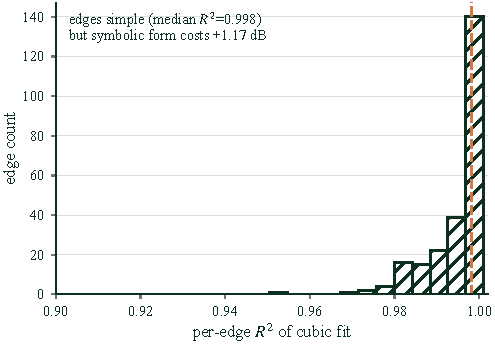
\includegraphics[width=\columnwidth]{fig_interp.pdf}
\caption{Interpretability audit on the DPD KAN. The learned edges are simple (a cubic fits
with median $R^2=0.998$), but distilling them into that symbolic form costs $1.17$~dB of
NMSE: the interpretable model is not the performant one.}
\label{fig:interp}
\end{figure}

% ============================================================================
\section{Ablations: Stress-Testing the Comparison}\label{sec:abl}
% ============================================================================
A single matched-budget comparison could be unfair to KANs in ways that a proponent would
rightly object to: perhaps the budget is too small, the KAN is under-tuned, the data too
plentiful, or the operating point unrepresentative. We therefore run four ablations, each
designed to give the KAN its best shot, and report the honest crossovers they reveal.

\emph{Budget sweep (Fig.~\ref{fig:budget}).} We sweep the DPD parameter budget from about
$0.8$k to $9$k. The MLP-over-KAN ordering persists at every budget, and the gap does not
close: the Fourier-KAN improves with budget but tracks below the MLP, and the spline-KAN
plateaus near $-14$~dB and stops improving. Giving the KAN more parameters of the same kind
does not rescue it here.

\emph{KAN and MLP hyperparameters (Tables~\ref{tab:kanhp} and~\ref{tab:mlphp}).} Fairness
demands that if we tune the KAN, we tune the MLP too. We do both. Increasing the Fourier basis
order to $K=8$ raises the Fourier-KAN to $\input{claims/dpd_fkan_k8_nmse}$~dB at
$\input{claims/dpd_fkan_k8_params}$ parameters, and spectral richness, not width, is the lever.
But the MLP is not fixed either: sweeping its depth and activation
(Table~\ref{tab:mlphp}), a three-layer MLP reaches $\input{claims/mlp_best_2330_nmse}$~dB at
the default budget, beating every matched-budget KAN there, and $\input{claims/mlp_tuned_k8budget_nmse}$~dB
at the larger $K=8$ budget. So the Fourier-KAN's regression win survives a \emph{symmetrically}
tuned MLP, but only by $\input{claims/k8_vs_tuned_mlp_margin}$~dB, down from $0.6$~dB against
the untuned MLP: a real but thin advantage, and only at the larger budget. This is the flip
side of the capacity-confound argument: just as an unmatched KAN can win for the wrong reason,
a well-chosen KAN can win for the right one, and only a matched, symmetrically tuned comparison
tells them apart.

\begin{table}[t]
\centering
\caption{Symmetric MLP sweep on DPD at the default budget ($5$ seeds). A tuned three-layer MLP
is the strongest matched-budget model, so the KAN is not beaten by an untuned baseline. The
default 2-layer row ($-16.25$) is this sweep's own run; it matches Table~\ref{tab:dpd}'s
$-16.27$ within seed noise.}
\label{tab:mlphp}
\begin{tabular}{lrr}
\toprule
MLP configuration & Params & NMSE [dB] $\downarrow$ \\
\midrule
$1$ layer, ReLU  & $2329$ & $-15.22\pm0.14$ \\
$2$ layer, ReLU (default) & $2354$ & $-16.25\pm0.08$ \\
$2$ layer, GELU  & $2354$ & $-14.48\pm0.22$ \\
$2$ layer, tanh  & $2354$ & $-15.78\pm0.13$ \\
$3$ layer, ReLU  & $2389$ & $\mathbf{-16.72\pm0.17}$ \\
$4$ layer, ReLU  & $2277$ & $-16.60\pm0.10$ \\
\bottomrule
\end{tabular}
\end{table}

\emph{Sample efficiency (Fig.~\ref{fig:samples}).} A distinct claimed KAN strength is
data efficiency. It holds here: with $1$k and $4$k training examples the Fourier-KAN beats
the matched MLP (paired differences $\input{claims/dpd_lowdata_kan_diff_1k}$ and
$\input{claims/dpd_lowdata_kan_diff_4k}$~dB, intervals excluding zero), and the ordering
inverts only once data is plentiful ($+\input{claims/dpd_highdata_mlp_diff}$~dB at the full
set). A KAN is a reasonable choice when labeled data is the binding constraint.

\emph{SNR sweep (Fig.~\ref{fig:snr}).} Finally we resolve the AMC accuracy by SNR instead of
aggregating over a band. The convolutional baseline leads at every SNR. Among the flat
models, the MLP is best only at low SNR; the spline-KAN overtakes it above about
$\input{claims/snr_crossover_db}$~dB (reaching $\input{claims/amc_kanspline_snr10}$ versus the
MLP's $\input{claims/amc_mlp_snr10}$ at $10$~dB), and over the \emph{full} SNR range the
spline-KAN is the best flat model ($\input{claims/amc_kanspline_fullrange}$ versus
$\input{claims/amc_mlp_fullrange}$). The aggregate ranking is thus an artifact of which band
one reports, which is the saturated-benchmark problem in a subtler form: not only can a band
be too easy, it can be chosen (even inadvertently) to favor one model.

\begin{figure}[t]
\centering
\includegraphics[width=\columnwidth]{fig_dpd_budget.pdf}
\caption{DPD budget sweep. The MLP leads at every budget; the Fourier-KAN improves but
tracks below it, and the spline-KAN plateaus. More same-kind parameters do not close the gap.}
\label{fig:budget}
\end{figure}

\begin{table}[t]
\centering
\caption{DPD KAN hyperparameter sweep (5 seeds). A richer Fourier basis
($K{=}8$, $-17.14$~dB at $4634$ params) beats even a symmetrically tuned MLP
($-16.95$~dB at that budget), but by only $0.19$~dB (see Table~\ref{tab:mlphp}).}
\label{tab:kanhp}
\begin{tabular}{llrr}
\toprule
Variant & Setting & Params & NMSE [dB] $\downarrow$ \\
\midrule
Fourier & $K=2$ & $1178$ & $-14.42\pm0.05$ \\
Fourier & $K=4$ & $2330$ & $-15.54\pm0.09$ \\
Fourier & $K=8$ & $4634$ & $\mathbf{-17.14\pm0.12}$ \\
spline  & grid $4$  & $1152$ & $-13.03\pm0.15$ \\
spline  & grid $6$  & $1440$ & $-14.04\pm0.13$ \\
spline  & grid $10$ & $2016$ & $-15.09\pm0.09$ \\
\bottomrule
\end{tabular}
\end{table}

\begin{figure}[t]
\centering
\includegraphics[width=\columnwidth]{fig_dpd_samples.pdf}
\caption{DPD sample efficiency. The Fourier-KAN beats the matched MLP when training data is
scarce ($\le 4$k examples); the ordering inverts only once data is plentiful.}
\label{fig:samples}
\end{figure}

\begin{figure}[t]
\centering
\includegraphics[width=\columnwidth]{fig_amc_snr.pdf}
\caption{AMC accuracy resolved by SNR. The CNN leads throughout; among flat models the MLP
wins only at low SNR, while the spline-KAN overtakes it above $\sim 2$~dB. Reporting a single
band hides this crossover.}
\label{fig:snr}
\end{figure}

% ============================================================================
\section{Computational Cost: The Efficiency Illusion}\label{sec:compute}
% ============================================================================
Matching parameter count, the axis on which KAN ``efficiency'' is usually claimed, hides the
axis that matters for deployment: compute. A KAN edge evaluates a spline or a truncated
Fourier series where an MLP edge evaluates a single multiply-add, so at equal parameters a KAN
does substantially more work. Counting multiply-adds per layer,
\begin{align}
C_{\mathrm{MLP}} &= 2\,d_{\mathrm{in}}d_{\mathrm{out}}, \label{eq:cmlp}\\
C_{\mathrm{KAN}}^{\mathrm{F}} &= 2K\,d_{\mathrm{in}}d_{\mathrm{out}} + \kappa\,(2K)\,d_{\mathrm{in}}, \label{eq:ckanf}\\
C_{\mathrm{KAN}}^{\mathrm{S}} &= (G{+}k)\,d_{\mathrm{in}}d_{\mathrm{out}} + \rho\,d_{\mathrm{in}}, \label{eq:ckans}
\end{align}
where $\kappa$ is the cost of a $\cos/\sin$ pair and $\rho$ that of the B-spline recurrence.
Two effects compound: the basis multiplies the connectivity term by $2K$ or $G{+}k$, and the
transcendental or recurrence terms add fixed per-edge overhead that no parameter count reflects.
The parameter budget absorbs the multiplicative factor by shrinking the hidden width, but the
per-edge overhead does not shrink with it; it reappears as latency.

Table~\ref{tab:compute} measures it. At the \emph{same} parameter budget, inference is
$\input{claims/compute_dpd_fkan_slowdown}\times$ to $\input{claims/compute_dpd_skan_slowdown}\times$
slower for the KANs than for the matched MLP on the regression models, and
$\input{claims/compute_amc_fkan_slowdown}\times$ to $\input{claims/compute_amc_skan_slowdown}\times$
slower on the classification models, with the canonical spline-KAN the most expensive by far.
So even in the regimes where a KAN edges out the MLP on accuracy, it pays with an order of
magnitude more compute per inference, and a practitioner optimizing performance per FLOP or per
millisecond, the realistic constraint at a base station or on an edge device, would not choose
it. ``Fewer parameters'' is the wrong metric; matched-parameter is already generous to the KAN.

\begin{table}[t]
\centering
\caption{Compute at matched parameters. Inference time per batch (256) and slowdown versus the
matched MLP. KANs cost far more compute for the same parameter count.}
\label{tab:compute}
\begin{tabular}{llrr}
\toprule
Task & Model & Params & Infer.\ [ms] $\downarrow$ \\
\midrule
DPD & MLP           & $2354$  & $0.04$ \\
DPD & KAN, Fourier  & $2330$  & $0.27$ \\
DPD & KAN, spline   & $2280$  & $1.14$ \\
\midrule
AMC & CNN           & $5291$  & $25.2$ \\
AMC & MLP           & $68651$ & $0.16$ \\
AMC & KAN, Fourier  & $68395$ & $0.74$ \\
AMC & KAN, spline   & $69420$ & $3.47$ \\
\bottomrule
\end{tabular}
\end{table}

% ============================================================================
\section{Discussion}\label{sec:discuss}
% ============================================================================
\subsection{A regime map}
Combining the regimes, the audit, and the ablations yields a compact map with three tiers.
\emph{Where KANs help:} at higher SNR in modulation classification, over the full SNR range,
in the low-data regime, and, with a richer basis, on smooth regression at matched capacity, a
KAN is the better flat model, sometimes by a clear margin. Their learnable edges are a real
tool, not a gimmick. \emph{Where they do not:} at the default budget and basis, at low SNR,
and with plentiful data, a same-size MLP is as good or better, so a KAN advantage is never
automatic. \emph{Where architecture matters more than either:} on structured I/Q
classification a small CNN with the right inductive bias beats every flat model by a wide
margin at a fraction of the parameters, so if the task has exploitable structure, the budget
is better spent on the prior than on the edge parameterization. Layered on top, KAN
interpretability is real but not free: the edges are genuinely simple, yet the symbolic
extraction that would make them interpretable costs more than a decibel.

\subsection{Interpreting the crossovers}
The crossovers are not random, and two mechanisms are consistent with all our observations,
though we frame them as hypotheses rather than claims. First, the KAN's per-edge nonlinearity
is most useful when the target relationship is a clean low-dimensional function of each input.
At high SNR the received constellation is sharp, so the mapping from I/Q samples to class is
close to a smooth geometric partition that per-edge functions can carve; at low SNR the same
flexibility fits noise, which is exactly where the more constrained MLP, and far more so the
translation-equivariant CNN, generalize better. This matches both the SNR crossover and the
low-data crossover: fewer, cleaner examples favor the model whose inductive bias is a smooth
univariate decomposition. Second, on the smooth regression task the benefit of the Fourier
basis grows with its order $K$ rather than with width, because a power-amplifier AM/AM curve
is well represented by a few harmonics; this is why $K{=}8$ overtakes the MLP while wider
low-$K$ KANs do not. Neither mechanism supports a blanket advantage; both predict a bounded
regime, which is what we measure.

\subsection{Why the literature reports sweeping wins}
Our results both confirm that KANs can win and explain why the reported wins are overstated.
A KAN with an unmatched budget, or with a richer basis than the MLP it is compared to, will
beat that MLP, and our own ablations reproduce exactly such a win once the KAN is tuned;
attributing it to ``the architecture'' rather than to the extra effective capacity is the
error. Likewise, a saturated benchmark makes every model tie so any fluctuation reads as a
win, and an aggregate over a favorable band hides the crossover we measured. The advantage
does not vanish under matched control, but it shrinks to a specific, honest set of regimes
rather than the blanket superiority usually claimed.

\subsection{Threats to validity}
We tested three regimes, two KAN variants, and one dataset per regime; a broader sweep (more
datasets, wavelet or Chebyshev KANs~\cite{wavkan,chebykan}, larger budgets) would refine the
regime boundaries, and we release the harness to make that cheap. The DPD PA is simulated,
though from a standard non-polynomial model, so the classical baseline is not privileged; a
measured PA would strengthen the regression result. The AMC study is capped in sample count
for tractability. Because our conclusions are two-sided, the main risk is mislocating a
boundary rather than a hidden global winner: every reported crossover has intervals that
exclude zero, and the interpretability cost was measured directly rather than inferred.

\subsection{Future work}
Three extensions would sharpen the map. First, a \emph{systematic audit} of the recent
KAN-in-wireless literature against the six-point checklist of Section~\ref{sec:discuss}: our
results predict that the reported efficiency wins will correlate with unmatched capacity,
saturated benchmarks, or unreported seeds, and a structured survey scoring each paper on the
six criteria would test that prediction directly and quantify how widespread the confounds
are. Second, a full DPD linearization loop with ACPR and EVM on a \emph{measured} power
amplifier, replacing our forward Saleh model, would confirm whether the thin regression
crossover survives real memory and hysteresis effects. Third, extending the model set to
wavelet and Chebyshev KANs~\cite{wavkan,chebykan} and adding a real multimodal benchmark such
as DeepSense~6G~\cite{deepsense6g} would probe whether any KAN variant reverses the ordering on
a task with genuinely exploitable structure. The released harness is designed to make each of
these a small addition rather than a reimplementation.

\subsection{Practical guidance}
For a wireless practitioner: if the task has exploitable structure, spend the model budget on
the right inductive bias (a convolution, an unrolled algorithm) rather than on the edge
parameterization, which dominated every flat model here. Among flat models, reach for a KAN
when labeled data is scarce or when the operating regime is clean (high SNR), where it beat
the matched MLP, and tune its basis richness, not just its width; otherwise a same-size MLP
is a strong and simpler default. If interpretability is the goal, measure the accuracy cost of
the symbolic extraction rather than assuming it is free. The recurring discipline is to match
capacity and resolve the operating point before believing any architecture comparison.

\subsection{A reporting checklist}
The confounds we removed are cheap to check, and we distill them into a checklist a reviewer
or author can apply to any KAN-versus-baseline wireless claim:
\begin{enumerate}
\item \textbf{Matched capacity.} Are the KAN and its baseline sized to the same parameter
count, reported explicitly? An efficiency claim against a smaller-parameter baseline is not
evidence about the architecture.
\item \textbf{Non-saturated benchmark.} Is the reported operating point one where models are
below the ceiling? If every model exceeds $\sim\!99\%$, the comparison is uninformative.
\item \textbf{Resolved operating point.} Is accuracy resolved by SNR (or the relevant axis)
rather than aggregated over a band that may favor one model, as our crossover shows?
\item \textbf{Multiple seeds with intervals.} Is the claim supported by a paired difference
with a confidence interval that excludes zero, not a single-seed number?
\item \textbf{Strong baseline.} Is the baseline the one a practitioner would use (a CNN for
I/Q, a memory polynomial for DPD), not a deliberately weak MLP?
\item \textbf{Interpretability with fidelity.} If interpretability is claimed, is the accuracy
cost of the symbolic extraction measured, not just a plot of a few edges?
\end{enumerate}
Every ``win'' we could not reproduce under matched control failed at least one of these
checks; every genuine KAN win we found survives all six.

% ============================================================================
\section{Reproducibility}\label{sec:repro}
% ============================================================================
Every number in this paper is produced by a script and checked against a machine-readable
claims file. The harness (\texttt{harness.py}) implements the KAN variants, the MLP, the
matched-capacity sizing, the training loop, and the bootstrap statistics; \texttt{exp\_dpd.py},
\texttt{exp\_amc.py}, and \texttt{exp\_interp.py} produce the main tables and
Figs.~\ref{fig:dpd}--\ref{fig:interp}, and \texttt{abl\_dpd.py} and \texttt{abl\_amc.py}
produce the ablations (Table~\ref{tab:kanhp}, Figs.~\ref{fig:budget}--\ref{fig:snr}), each
from its own result CSV. The RML2016.10a dataset is public~\cite{oshea2016gnuradio}. We list,
for each table and figure, the exact script and CSV that generate it, and we fix all random
seeds. The code and a \texttt{claims.json} single-source-of-truth are released so that a
reader can regenerate the results and verify the paper's numbers against the CSVs. The full
code, result CSVs, and the claims file are available at
\url{https://github.com/haodpsut/kan-wireless-benchmark}.

% ============================================================================
\section{Conclusion}\label{sec:concl}
% ============================================================================
We asked when Kolmogorov--Arnold networks help in wireless, and answered by measurement.
Under a parameter-matched, multi-seed, non-saturated protocol, the honest answer is
two-sided: KANs are competitive and win in specific regimes, at higher SNR in modulation
classification, in the low-data regime, and with a richer basis on smooth regression, but
they never dominate, are beaten decisively by the right inductive bias on structured tasks,
lose to a same-size MLP at the default budget and at low SNR, and carry an interpretability
cost of more than a decibel to extract. The sweeping ``efficiency wins'' reported in the
wireless KAN literature are consistent with unmatched capacity and saturated or favorably
chosen benchmarks rather than with a blanket architectural advantage. We hope the regime
map, the protocol, and the released harness make the next such claim easier to place, and to
check, before it is believed.

\bibliographystyle{IEEEtran}
\bibliography{refs}

\end{document}
